\documentclass[11pt,a4paper]{article}
%%%%%%%%%%%%%%%%%%%%%%%%%%%%%%%%%%%%%%%%%%%%%%%%%%%%%%%%%%%%%%%%%%%%%%%%%%%%%%%%%%%%%%%%%%%%%%%%%%%%%%%%%%%%%%%%%%%%%%%%%%%%%%%%%%%%%%%%%%%%%%%%%%%%%%%%%%%%%%%%%%%%%%%%%%%%%%%%%%%%%%%%%%%%%%%%%%%%%%%%%%%%%%%%%%%%%%%%%%%%%%%%%%%%%%%%%%%%%%%%%%%%%%%%%%%%
\usepackage{float}
\usepackage{graphicx,amsmath}
\usepackage{hyperref}

\setcounter{MaxMatrixCols}{10}
%DISTAL{OutputFilter=LATEX.DLL}
%TCIDATA{Version=5.50.0.2960}
%TCIDATA{Codepage=1252}
%TCIDATA{<META NAME="SaveForMode" CONTENT="1">}
%TCIDATA{BibliographyScheme=Manual}
%TCIDATA{LastRevised=Tuesday, October 23, 2018 17:45:13}
%TCIDATA{<META NAME="GraphicsSave" CONTENT="32">}

\renewcommand{\floatpagefraction}{.9}
\renewcommand{\textfraction}{.1}
\oddsidemargin 0cm \evensidemargin 0cm \textwidth 17cm \topmargin
-1.5cm \textheight 23.5 cm
\newcommand{\pdf}[3]{
\begin{figure}[tp]
\begin{center}
\includegraphics[height=#1,keepaspectratio]{#2.pdf}
\end{center}
\caption{#3} \label{#2}
\end{figure}
}
\newcommand{\pdfstack}[4]{
\begin{figure}[p]
\begin{center}
\includegraphics[height=4in,keepaspectratio]{#1.pdf}
\end{center}
\caption{#2} \label{#1}
\begin{center}
\includegraphics[height=4in,keepaspectratio]{#3.pdf}
\end{center}
\caption{#4} \label{#3}
\end{figure}
}
%\input{tcilatex}
\begin{document}



\begin{center}
\textbf{Ecole Polytechnique}

\bigskip

\textbf{Eco 432 - Macro\'{e}conomie}

\bigskip

\textbf{PC 3. La prime salariale associée aux études supérieures}

\hspace{1.0in}
\end{center}


\begin{center}
\textbf{Exercise 1}
\end{center}





\textbf{Solution}: L'entreprise maximise les profits $Y-w_HH-w_LL$. Les deux conditions de premier ordre nous donnent la demande de $H$ et la demande de $L$: \begin{equation}
    w_H=(1-\alpha) A_H^{1-\alpha}H^{-\alpha}A_L^{\alpha}L^{\alpha}\label{uno}
\end{equation}

\begin{equation}
    w_L=(\alpha) A_H^{1-\alpha}H^{1-\alpha}A_L^{\alpha}L^{\alpha-1}
\end{equation}

Autrement dit, étant donné les salaires (que les entreprises considèrent comme donnés), ces deux équations nous donnent implicitement la demande de H et de L. Comme on s'y attend, si le salaire baisse, la demande augmente. La prime salariale associée aux études supérieures est 
\begin{equation}
\frac{w_H}{w_L}=\frac{1-\alpha}{\alpha}\frac{L}{H}
\end{equation}
 Lorsque $\alpha=0.5$, \begin{equation}
    w_H/w_L=L/H
\end{equation}
Étant donné qu'une plus grande scolarisation a augmenté $H/L$, le modèle prédirait une diminution de la prime salariale, ce qui n'est pas ce que nous avons observé dans les données .


Pour mieux comprendre l'effet de $H/L$ sur la prime salariale, regardons l'effet de H/L sur $w_H$ et $w_L$. D'après l'équation (\ref{uno}), lorsque H/L augmente, le salaire des personnes hautement qualifiées $w_H$ diminue. Dessinez l'offre et la demande sur les deux marchés (haute et basse qualification). Supposons que l'offre est verticale sur les deux marchés. Supposons que H augmente (et que L reste constant). L'offre de travailleurs hautement qualifiés est plus importante, mais la demande de travailleurs hautement qualifiés est inchangée. En conséquence, $w_H$ doit baisser.  Qu'arrive-t-il à $w_L$ ?
Nous avons que $w_L$ augmente parce que les individus peu qualifiés deviennent plus productifs lorsqu'il y a plus d'individus hautement qualifiés : cela découle du fait que la dérivée croisée $F_{HL}>0$.

\begin{center}
\textbf{Exercise 2}
\end{center}



%Affirmer que lorsque $\sigma$ tend vers zéro, H et L deviennent des compléments parfaits (les deux inputs sont utilisees
%ensemble et il difficile de remplacer un input par l’autre); when instead $\sigma$ goes to infinity, H and L become perfect substitutes.\footnote{Facteurs parfaitement substituables. On dit que des facteurs sont parfaitement substituables si, pour se dispenser d’une unité d’un des deux facteurs, il faut toujours la même quantité additionnelle de l’autre facteur, pour un même niveau de production} 

%the shape of the isoquant of the production function (\ref{ces2}). 

\bigskip

(i) \textbf{Solution}: Pour dessiner l'isoquant, nous calculons comment la pente de l'isoquant varie avec $\sigma$. Calculons la pente. Étant donné une fonction $Y=F(H,L)$ calculer le differentielle totale: 

\begin{equation}
    dY=\frac{\partial F}{\partial H}dH+\frac{\partial F}{\partial L}dL
\end{equation}
Le long d'un isoquant, par définition l'output ne varie pas: $dY=0$.
Alors, la pente de l'isoquant est

\begin{equation}
    \frac{dL}{dH}= -\frac{\frac{\partial F}{\partial H}}{\frac{\partial F}{\partial L}}
\end{equation}
En utilisant les conditions du premier ordre, la valeur absolue de la pente est:
\begin{equation}
   \mid \frac{dL}{dH} \mid \ &=&\frac{w_H}{w_L}
\end{equation}



\begin{equation}
     \mid \frac{dL}{dH} \mid \ =\frac{\left[  (A_L L)^{\frac{\sigma -1}{\sigma }}+  (A_HH)^{\frac{\sigma -1}{%
\sigma }}\right] ^{\frac{\sigma }{\sigma -1}-1}A_H^{ ^{\frac{\sigma -1}{\sigma }} }H^{\frac{\sigma -1}{\sigma }-1}}{\left[  (A_L L)^{\frac{\sigma -1}{\sigma }}+  (A_HH)^{\frac{\sigma -1}{%
\sigma }}\right] ^{\frac{\sigma }{\sigma -1}-1}A_L^{^{\frac{\sigma -1}{\sigma }}}L^{\frac{\sigma -1}{\sigma }-1}}
\end{equation}


On obtient: 
\begin{equation}
    \mid \frac{dL}{dH} \mid =(\frac{A_H}{A_L})^{\frac{\sigma -1}{\sigma}} (\frac{H}{L})^{-\frac{1} {\sigma}}
\end{equation}

On distingue trois cas.  Quand $\sigma$ tend vers 1, la pente de l'isoquant converge à la pente   de l'isoquant de le fonction Cobb-Douglas de l'exercice 1 quand $\alpha=0.5$.

Lorsque $\sigma$ tend vers 0,  la pente converge vers

\begin{equation}
   \mid \frac{dL}{dH} \mid=\left(\frac{A_H H}{A_L L}\right)^{-\infty} 
\end{equation}
Cela signifie que la pente est soit nulle (lorsque $A_L L<A_HH$) soit infinie (lorsque $A_L L>A_HH$). Dans ce cas, l'isoquant a un coude, ce qui signifie que les deux facteurs sont peu substituables : les deux facteurs doivent être utilisées dans des proportions fixes.
\begin{equation}
   \lvert \frac{dL}{dH} \mid =\frac{A_H}{A_L}^{\frac{\sigma -1}{\sigma}} (\frac{H}{L})^{-\frac{1} {\sigma}}
\end{equation}

Pour déduire la forme de l'isoquant lorsque $\sigma$ tend vers $\infty$, on peut directement regarder la fonction de production. La fonction CES devient
\begin{equation}\label{ces2}
Y_t=\left[  (A_L L)+  (A_HH)\right] 
\end{equation}

Dans ce cas  \begin{equation}
    \frac{dL}{dH}=\frac{A_H }{A_L}
\end{equation}


Les deux inputs sont des substituts parfaits et la pente est constante.  \bigskip

%In paerticular, $\sigma$ determines the shape of the isoquant in the space (H,L).  

%In  the context of the substitution between college and non-college workers, a relatively high elasticity of substitution is plausible.  Most estimates of $\sigma$ are somewhere between 1.4 and 2.

%In the space (L,H) draw the isoquant, that is, draw the contour line drawn through the set of points at which the same quantity of output is produced while changing the quantities of $H$ and $L$. The absolute value of the slope of the isoquant, or the MRTS is $(MP_H)/(MP_L)$.  
%Show that when $\sigma$ goes to 1, the isoquant converges to the slope of the isoquant of the Cobb-Doug;as } (\ref{cd}) with $\alpha=0.5$. When instead, $\sigma$ goes to zero, the isoquant have a kink (the solope of the sioquant is 



\bigskip
(ii) \textbf{Solution}:  \begin{equation}\label{due}
    \frac{w_H}{w_L} = \frac{A_H}{A_L}^{\frac{\sigma -1}{\sigma}} (\frac{H}{L})^{-\frac{1} {\sigma}}
\end{equation}

Le prime salariale dépend maintenant de H/L mais aussi de la  technologie.  Pour un ratio technologique $A_H/A_L$ donné, l'augmentation de l'offre relative de travailleurs hautement qualifiés réduit la prime salariale avec une élasticité de $-1/\sigma$.\footnote{Lorsque $\sigma$ est  grand, les fonctions de demande sont assez plates puisque le produit marginal est constant : les salaires réagissent peu aux variations de l'offre.} Cependant,  dans les données, $A_H/A_L$ a probablement augmenté: la numérisation et les technologies de l'information augmentent la productivité des travailleurs qualifiés plus que la productivité des travailleurs peu qualifiés. Lorsque $\sigma>1$, l'augmentation de
$A_H/A_L$ augmente la prime salariale. Les économistes (cf. Goldin et Katz, 2008) estiment que la hausse de $A_H/A_L$ ("skill-biased technological change") a été suffisamment forte pour compenser l'effet dû à la hausse de H/L.\footnote{La figure 1 montre que la scolarisation a quelque peu plafonné récemment aux Etats-Unis, ce qui a renforcé l'effet du changement technologique.} Il est intéressant de remarquer que lorsque $0<\sigma \leq 1$, le modèle n'a aucune chance de reproduire l'augmentation de la prime salariale. Pour comprendre cela, supposons que H et L sont très complémentaires et doivent être utilisés en proportion fixe. Dans ce cas, lorsque H devient plus productif, il est moins rémunéré en termes relatifs ! Ce résultat semble paradoxal mais reflète qu'une fois que H devient plus productif, l'entreprise en a moins besoin pour produire un objectif de production donné. 
\begin{figure}[th]
\centering
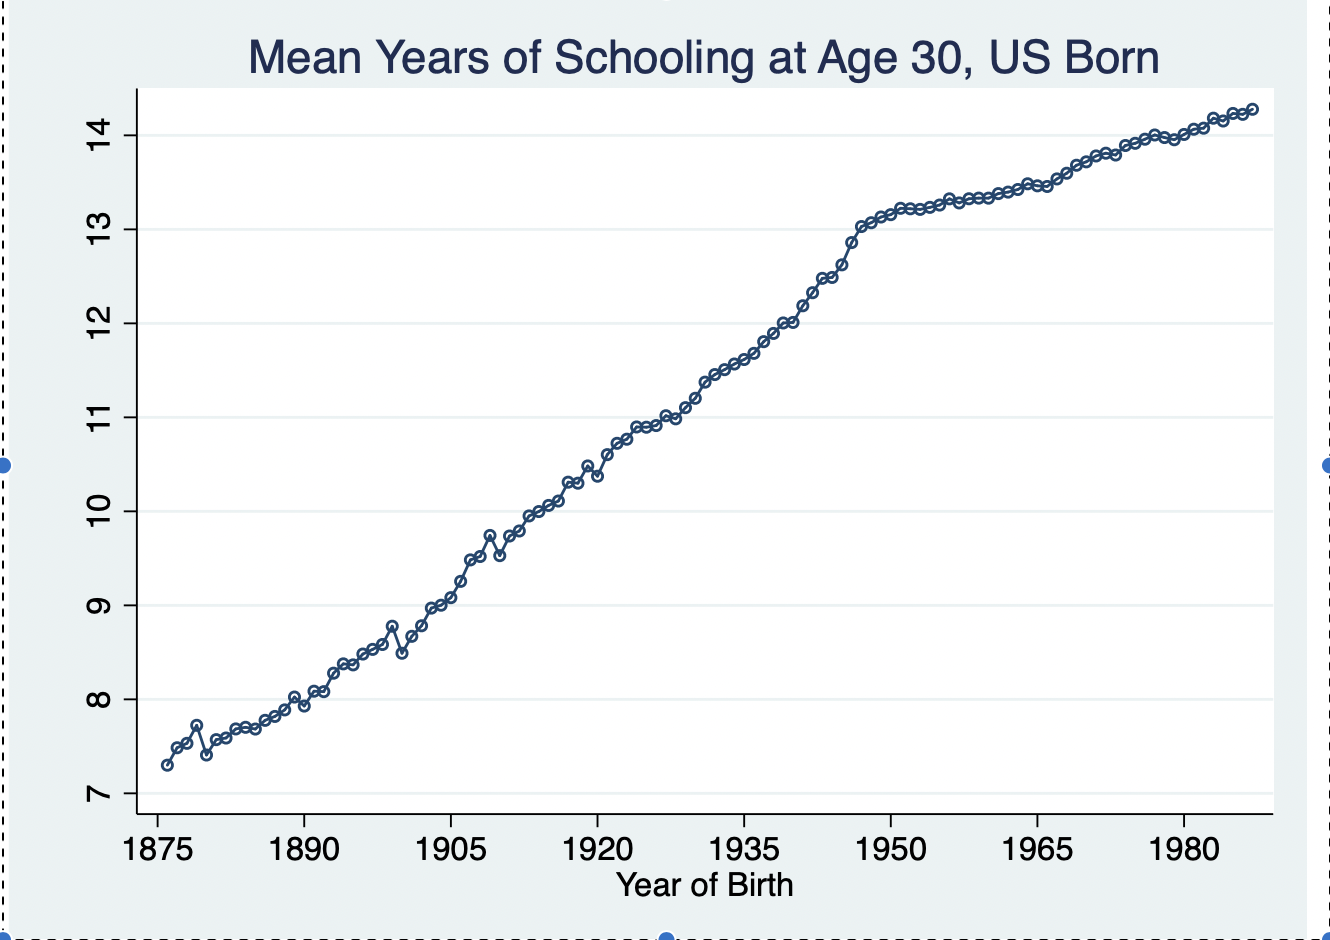
\includegraphics[keepaspectratio=true, scale=0.3, clip = true]{PLAT.png}
\caption{\textbf{Scolarisation}}
\label{fig:1.4}
\end{figure}
 

    
Peut-on utiliser ce modèle pour expliquer la baisse des salaires peu qualifiés en termes absolus ? La réponse, comme nous allons le montrer, est non. En fait, nous montrerons ci-dessous que des $H/L$ ou $A_H$ plus élevés auraient augmenté les salaires des travailleurs peu qualifiés. En fait, sous la technologie CES nous avons : \begin{equation}
        \frac{\partial w_L}{\partial A_H} >0 
    \end{equation}
  et  \begin{equation}
        \frac{\partial w_L}{\partial (H/L)} >0 
    \end{equation}
    
Pour voir cela, nous calculons le salaire de la main-d'œuvre peu qualifiée :
    
    \begin{equation}
        w_L=A_L^{\frac{\sigma-1}{\sigma}} \left[A_L^{\frac{\sigma-1}{\sigma}} +A_H^{\frac{\sigma-1}{\sigma}}(\frac{H}{L})^{\frac{\sigma-1}{\sigma}}\right]^{^{\frac{\sigma}{\sigma-1}-1}}
    \end{equation}
    
En prenant la dérivée par rapport à $A_H$ on a :
    
    \begin{equation}
             \frac{\partial w_L}{\partial A_H}= \frac{1}{\sigma-1} \frac{\sigma-1}{\sigma} A_L^{\frac{\sigma-1}{\sigma}} \left[A_L^{\frac{\sigma-1}{\sigma}} +A_H^{\frac{\sigma-1}{\sigma}}(\frac{H}{L})^{\frac{\sigma-1}{\sigma}}\right]^{^{\frac{\sigma}{\sigma-1}-2}}A_H^{\frac{\sigma-1}{\sigma}-1}(\frac{H}{L})^{\frac{\sigma-1}{\sigma}}
             \end{equation}

Puisque les termes avec $\sigma-1$ s'annulent, les termes restants sont tous positifs (puisque $A_L$, $A_H$, $H$ et $L$ sont positifs):  la dérivée est bien positive. Les travailleurs peu qualifiés bénéficient en termes absolus lorsque les travailleurs hautement qualifiés deviennent plus productifs. De la même manière, on peut montrer que la dérivée par rapport à $H/L$ est positive. Ainsi, la seule façon d'obtenir une baisse de $w_L$ est d'avoir une régression technologique, ce qui est assez invraisemblable.


\begin{center}
\textbf{Exercise 3} 
\end{center}


(1) \textbf{Solution:} Les salaires sont égaux aux productivités marginales :

\begin{equation}\label{tre}
    w_R=\frac{\partial Y}{\partial L_R}=(1-\beta)\theta^{-\beta}
\end{equation}
\begin{equation}\label{wn}
    w_N=\frac{\partial Y}{\partial L_N}=\beta \theta ^{1-\beta}
\end{equation}


Puisque $w_R=\rho$, en utilisant  (\ref{tre}) on obtient: \begin{equation}\label{tet}
    \theta=(\frac{1-\beta}{\rho})^{1/\beta}
\end{equation}

\bigskip 
Il faut montrer que \begin{equation}\frac{\partial \ln w_N }{\partial \ln \rho}= \frac{\beta -1 }{\beta}<0
\end{équation}}

En utilisant (\ref{tet}) et (\ref{wn})
\begin{equation}
w_N = \beta (\frac{1-\beta}{\rho})^{\frac{1-\beta}{\beta}}
\end{equation}

En prenant des logs et en prenant la dérivée, on obtient le résultat recherché. Le progrès technologique baisse le salaire des emplois routiniers, mais il rend  les emplois non routiniers plus productifs car la dérivée croisée de la fonction de production est positive. 


Nous avons aussi
\begin{equation}\frac{\partial \ln (\theta) }{\partial \ln \rho}= -\frac{ 1 }{\beta}
\end{équation}}

Une baisse du prix du capital informatique augmente l'intensité  des tâches non routinières  dans la production.


\end{document}
%\begin{equation}
w_N =\frac{\partial Y}{\partial L_N}=(\frac{1-\beta}{\beta})^{1/\beta}
\end{equation}


\begin{equation}
\theta =(\frac{1-\beta}{\beta})^{1/\beta}
\end{equation}


\begin{equation}
\frac{w_N}{w_R}=\frac{\beta}{\1-\beta} (\frac{1-\beta}{\beta})^{1/\beta}
\end{equation}
Plusieurs études ont montré que
les opportunités d'emploi aux États-Unis et dans de nombreux pays se sont fortement polarisées
au cours des deux dernières décennies. D'une part, les opportunités d'emploi se multiplient
tant dans les professions hautement qualifiées que dans les professions peu qualifiées. D'un autre côté, les opportunités d'emploi sont réduites dans les professions moyennement qualifiées.
  (emplois de cols blancs et de cols bleus). Étant donné que les tâches routinières sont souvent effectuées par des travailleurs moyennement qualifiés, cet exercice peut aider à expliquer le phénomène de polarisation des opportunités d'emploi.

%Cheaper computers lead to a rise in routine inputs 
Also show that as computers become cheaper, $w_N/w_R$ increases:  \begin{equation}\frac{\partial \ln (w_N/w_R) }{\partial \rho}=- \frac{1}{\beta}
\end{equation}


Several studies have shown that the structure of
job opportunities in the United States and many countries has sharply polarized
over the past two decades, with expanding job opportunities
in both high-skill, high-wage occupations and low-skill, low wage occupations, coupled with contracting opportunities in
middle-wage, middle-skill white-collar and blue-collar jobs.

This model allows to provide some explanation.  A leading
explanation focuses on the consequences of ongoing automation and offshoring of middle-skilled “routine” tasks that
were formerly performed primarily by workers with moderate
education (a high school diploma but less than a four-year college degree). 

Autor et al, find that a secular growth in non-routine interactive/cognitive occupations, and declining employment in routine-intensive occupations (but also a secular decline in non-routine manual tasks (a bit surporising given growth in low-skill services). They also find that computerization is associated with reduced labor input of routine manual and routine cognitive tasks and
increased labor input of nonroutine cognitive tasks.

In
this case, the wages paid to high skilled workers cannot exceed the rental price (per efficiency
unit) of the machine, and declines in the price of the machine (or increases in its efficiency)
will lower the price of skilled workers.  



%Routine tasks can be accomplished by following explicit rules. Problem-solving and communication activities are “nonroutine”
%tasks. 



The production function (\ref{autor}) implies that computer capital substitutes for workers in carrying out routine tasks. 
At the same time, a greater quantity of computers increase the marginal product of nonroutine tasks. Finally, notice that routine and nonroutine tasks are themselves imperfect
substitutes. 


\begin{equation}
\theta =(\frac{1-\beta}{\beta})^{1/\beta}
\end{equation}


\begin{equation}
\frac{w_N}{w_R}=\frac{\beta}{\1-\beta} (\frac{1-\beta}{\beta})^{1/\beta}
\end{equation}

Each worker $i$ is endowed with productivity $(n_i,r_i)$, where $r_i$ is the productivity in performing routine tasks while $n_i$ is the productivity in performing non-routine tasks. Assume $0<r_i,n_i \leq 1.$ The wage per efficiency unit of routine (respectively non-routine) task
input is $w_R$ (respectively $w_N$).


Workers must choose whether to supply routine or non-routine tasks. Workers choose to supply routine tasks iff \begin{equation} w_Rr_i \geq  w_Nn_i \end{equation} Given $w_R$ and $w_N$, it is possible to compute the labour supply of routine and non-routine inputs. For instance, the total supply of routine inputs is $g(w_R,w_N)=\sum_i (r_i) \cdot  I (w_Rr_i <  w_Nn_i) $ where $I$  is an indicator function. The  total supply of non-routine inputs is $h(w_R,w_N)=\sum_i (n_i) \cdot  I (w_Rr_i \leq  w_Nn_i) $. 

Because there is perfect substitutability of routine tasks
and computer capital, the wage per efficiency unit of routine task
input is pinned down by the price of computer capital


\bigskip

(3) Show that an increase in the wage premium $w_N/w_R$ will raise labor supply to the non-routine occupation: ''marginal" workers  reallocate labor supply from routine to nonroutine task input.  
Thus, when $\rho$ declines the increase in $\theta $ is met entirely by an increase of computer capital.



Answer: 
\begin{equation}
\frac{w_H}{w_L}= \frac{  (A_L L)^{\alpha}  (A_H)^{1-\alpha} (1-\alpha) H^{-\alpha}}{  (A_L)^{\alpha}  (A_H H)^{1-\alpha}\alpha L^{\alpha-1}}
\end{equation}


\begin{equation}
\frac{w_H}{w_L}= \frac{   (1-\alpha)  }{ \alpha }\frac{L}{H}
\end{equation}

The effect of technological progress: Technology progress (higher $A_L$ and $A_H$) has no effect on the college premium (the ratio $w_H/w_L$ but it raises both $w_L$ and $w_H$. Of course, if for instance  $A_L$ increases, one expects the marginal product of low skill labour $w_L$ to increase. Moreover, if $A_H$ increases, low skill benefits as well because in the Cobb-Douglas the marginal product of $L$ increases if $H$ becomes more productive. 

\medskip

The effect of H/L:  The model predicts that if $H/L$ increases, then the college premium decreases (which is not what we observed). The increase in the relative supply of high skilled worker will cause firms to reassign some ’tasks’ performed by low skilled workers to high skilled workers, thereby lowering the marginal productivity of high skilled workers and hence their relative wage. 

%https://www.oecd.org/skills/piaac/Skills%20volume%201%20(eng)--full%20v12--eBook%20(04%2011%202013).pdf 


 \begin{equation}
w_L= \frac{ \partial Y_t}{\partial L}= (A_L)^{\frac{\sigma -1}{\sigma }} L^{-1/\sigma} \left[ (A_L L)^{\frac{\sigma -1}{\sigma }}+(A_HH)^{\frac{\sigma -1}{%
\sigma }}\right] ^{\frac{1}{\sigma -1}}=
\end{equation}
 
 
  \begin{equation}
w_L=  (A_L)^{\frac{\sigma -1}{\sigma }} L^{-1/\sigma}  L^{1/\sigma} \left[ (A_L)^{\frac{\sigma -1}{\sigma }}+A_H^{\frac{\sigma -1}{%
\sigma }} (\frac{ H}{L})^{\frac{\sigma -1}{%
\sigma }}\right] ^{\frac{1}{\sigma -1}}=
\end{equation}



  \begin{equation}
w_L=  (A_L)^{\frac{\sigma -1}{\sigma }}  \left[ (A_L)^{\frac{\sigma -1}{\sigma }}+A_H^{\frac{\sigma -1}{%
\sigma }} (\frac{ H}{L})^{\frac{\sigma -1}{%
\sigma }}\right] ^{\frac{1}{\sigma -1}}=
\end{equation}


Answer:   \begin{equation}
\frac{w_H}{w_L}=   \frac{\frac{ \partial Y_t}{\partial H}}{\frac{ \partial Y_t}{\partial L}} = (\frac{A_H}{A_L})^{\frac{\sigma -1}{\sigma }} (\frac{H}{L})^{-1/\sigma}=
\end{equation}
\begin{center}


Everything else equal, as the fraction of skilled workers in the labor force increases, the wages of unskilled workers should increase. In other words, skilled and unskilled workers are ’Q-complements’: a greater quantity of the one increases the marginal product of the other.

%As the fraction of high skill workers in the labor force increases, the low skill wage should increase. This is an implication of imperfect substitution between high and low skill workers. An increase in the fraction (or relative supply) of high skill workers increases the demand for the services of low skill workers, pushing up their unit wage





Answer: This result is intuitive but will also turn out to be important: technological improvements of any sort will lead to higher wages for both skill groups in the canonical model (also following from q-complementary). Thus unless there is “technical regress,” the canonical model cannot account for declining (real) wages of a factor whose supply is not shifting outward.





Answer:   \begin{equation}
\frac{w_H}{w_L}=  (\frac{A_H}{A_L})^{\frac{\sigma -1}{\sigma }} (\frac{H}{L})^{-1/\sigma}=
\end{equation}
\begin{center}

There is a simple log linear relationship between the skill premium and the relative supply of skills as measured by H/L.

then an increase in t
 \bigskip
 \begin{equation}\label{ces}
Y_t=\left[ (A_L L)^{\frac{\sigma -1}{\sigma }}+(A_HH)^{\frac{\sigma -1}{%
\sigma }}\right] ^{\frac{\sigma }{\sigma -1}}
\end{equation}
 (2) Show that $w_L$ is increasing in both $A_H$ and $A_L$. Interpret this result.  In the data low skill workers  (particularly low skill male)
have experienced significant real earnings declines over the last decades. Can this simple model explain this decline ? 
\bigskip


(3) Show that the wage premium $w_H/w_L$ is decreasing in $H/L$ and, assuming that $\sigma>1$, is increasing in the skill-bias of technology $A_H/A_L$. Interpret this result. This model indicates that the wage premium is determined by a race between the increase in the supply of skills and skill-biased technical change, which increases the relative demand for high skills.  This model helps explain why the wage premium has increased in the 70s, when there was a deceleration in the growth of college relative supply .

\bigskip

\begin{center}
    
\textbf{Exercise 3} 
\end{center}

The previous model assumes that output is a function of skills ($H$ and $L$) and does not distinguish between workers’ skills and job tasks. In reality, the assignment of skills to tasks is determined in equilibrium by labor supplies,
technologies, and task demands. For example, college graduate may perform analytical tasks when computers are expensive, but may be replaced by computers when computers become cheaper. 


An alternative approach to (\ref{ces}) is given by  the task-based approach:  skills do not directly produce
output, but workers apply
their skills to tasks in exchange for wages. Assume the following production function:

\begin{equation}\label{autor}
    Y=(L_R+K)^{1-\beta}(L_N)^{\beta}
\end{equation}
$\beta \in (0,1)$, where $L_R$ and $L_N$ are routine and nonroutine labor inputs (‘‘tasks") and $K$ is computer capital, all measured in efficiency units.  Routine tasks can be accomplished by following explicit rules. Problem-solving and communication activities are “nonroutine”
tasks. One efficiency unit of computer capital costs $\rho$.  



The production function (\ref{autor}) implies that computer capital substitutes for workers in carrying out routine tasks. 
At the same time, a greater quantity of computers increase the marginal product of nonroutine tasks. Finally, notice that routine and nonroutine tasks are themselves imperfect
substitutes. 

Each worker $i$ is endowed with productivity $(n_i,r_i)$, where $r_i$ is the productivity in performing routine tasks while $n_i$ is the productivity in performing non-routine tasks. Assume $0<r_i,n_i \leq 1.$ The wage per efficiency unit of routine (respectively non-routine) task
input is $w_R$ (respectively $w_N$).


Workers must choose whether to supply routine or non-routine tasks. Workers choose to supply routine tasks iff \begin{equation} w_Rr_i \geq  w_Nn_i \end{equation} Given $w_R$ and $w_N$, it is possible to compute the labour supply of routine and non-routine inputs. For instance, the total supply of routine inputs is $g(w_R,w_N)=\sum_i (r_i) \cdot  I (w_Rr_i <  w_Nn_i) $ where $I$  is an indicator function. The  total supply of non-routine inputs is $h(w_R,w_N)=\sum_i (n_i) \cdot  I (w_Rr_i \leq  w_Nn_i) $. 

Because there is perfect substitutability of routine tasks
and computer capital, the wage per efficiency unit of routine task
input is pinned down by the price of computer capital

\begin{equation}
    w_R=\rho
\end{equation}
As a result, technological progress in the capital sector, which leads to a decline in the price of computers,  lowers $ w_R$.

Define the ratio of routine to non-routine inputs in production:  


\begin{equation}
    \theta \equiv \frac{L_R + K}{L_N} 
\end{equation}


\bigskip

(1) Solve the problem of the representative firm and find the demand of routine and non-routine inputs. Express these demands as a function of $\theta$.  Using the first order-condition with respect to $L_R$, find $\theta$ as a function of $\rho$.


\bigskip

(2) Since routine and non-routine tasks are complementary inputs, a decline in the price of computing power unambiguously increases the marginal productivity of workers engaged in non-routine tasks. Show that \begin{equation}\frac{\partial \ln w_N }{\partial \rho}= \frac{\beta -1}{\beta}<0
\end{equation}
 Also show that as computers become cheaper, the wage premium increases:  \begin{equation}\frac{\partial \ln (w_N/w_R) }{\partial \rho}=- \frac{1}{\beta}
\end{equation}

\bigskip

(3) Show that an increase in the wage premium $w_N/w_R$ will raise labor supply to the non-routine occupation: ''marginal" workers  reallocate labor supply from routine to nonroutine task input.  
Thus, when $\rho$ declines the increase in $\theta $ is met entirely by an increase of computer capital.


\begin{figure}[th]
\centering
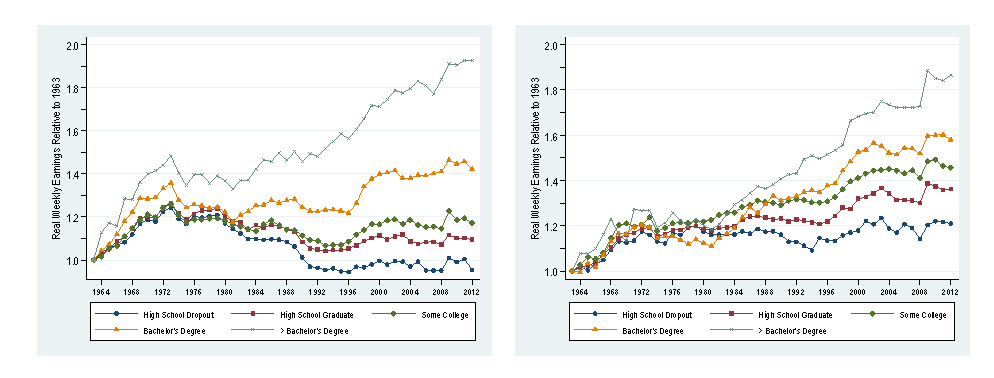
\includegraphics[keepaspectratio=true, scale=1.1, clip = true]{skills_premiumMW.pdf}
\caption{Change in Real Wage Levels of Full-Time Male (A) and female (B)
Workers by Education, 1963 - 2012, Autor 2014}
\label{fig:1.5}
\end{figure}

\end{document}

%w_Rr_i \geq  w_Nn_i
%the sum over the entire population  population endowments in ef��ciency units of routine and nonroutine tasks 


Workers are heterogenous: worker $i$ endowed with efficiencies (skills) given by  $E_i={r_i,n_1}$ where $n_i,r_i\in (0,1]$
Workers must choose whether to supply routine or non-routine tasks. Workers choose to supply routine tasks iff $w_Rr_i \geq  w_Nn_i$





Answer: We find that the saving rate is $s=\frac{\beta}{1+\beta}. $. 

Without capital markets, \begin{equation*} b^j_{t}=   sA (b^j_{t-1})^{\alpha}  \end{equation*}

and the steady state is $(sA)^{\frac{1}{1-\alpha}}$.

With perfect capital market, individuals choose the optimal size of the activity

\begin{equation*}k^{\ast}=\arg \max_{k}  Ak^{\alpha} -Rk\end{equation*}



\begin{equation*}A\alpha k^{\alpha-1}=R\end{equation*}


\begin{equation*} k^{\ast}=(\frac{A\alpha}{R})^{1/(1-\alpha)}\end{equation*}


Profits

\begin{equation*} \pi=   A(k^{\ast})^{\alpha} -Rk^{\ast}\end{equation*}


\begin{equation*} m^j=   \pi + R b^j_{t-1} \end{equation*}

\begin{equation*} b^j_{t}=   s(\pi + R b^j_{t-1}) \end{equation*}

The transition is linear, with slope less than one. 

Without capital markets, \begin{equation*} b^j_{t}=   sA (b^j_{t-1})^{\alpha}  \end{equation*}

Suppose now that the production technology is: \begin{equation} y^j_t=A(k^j_t)^{\alpha} \ \  if \ \ k^j_t > \underline{k} \end{equation} 
 \begin{equation}  y^j_t=\underline{w} \ \ if \ \ k^j_t \leq \underline{k} \end{equation} 
Assume that R is not too big, so that profits $\pi$ are more than $\underline{w}$.  If capital markets are perfect, everybody chooses to use the CD technology


\begin{equation*} b^j_{t}=   s(\pi + R b^j_{t-1}) \end{equation*}

If  they are not perfect, we have 
 \begin{equation} b^j_{t}=   sA (b^j_{t-1})^{\alpha}  if \ \ k^j_t > \underline{k} \end{equation} 
 \begin{equation}  b^j_{t}=   s\underline{w} + (b^j_{t-1}) \ \ if \ \ k^j_t \leq \underline{k} \end{equation} 


Since the subsistence activity needs no capital, any capital that an individual owns is part of total income, but there is no interest earned on it, as capital markets are assumed to be absent.

\bigskip 

Expercise 2

 \begin{equation}
w_L= \frac{ \partial Y_t}{\partial L}= (A_L)^{\frac{\sigma -1}{\sigma }} L^{-1/\sigma} \left[ (A_L L)^{\frac{\sigma -1}{\sigma }}+(A_HH)^{\frac{\sigma -1}{%
\sigma }}\right] ^{\frac{1}{\sigma -1}}=
\end{equation}
 
 
  \begin{equation}
w_L=  (A_L)^{\frac{\sigma -1}{\sigma }} L^{-1/\sigma}  L^{1/\sigma} \left[ (A_L)^{\frac{\sigma -1}{\sigma }}+A_H^{\frac{\sigma -1}{%
\sigma }} (\frac{ H}{L})^{\frac{\sigma -1}{%
\sigma }}\right] ^{\frac{1}{\sigma -1}}=
\end{equation}



  \begin{equation}
w_L=  (A_L)^{\frac{\sigma -1}{\sigma }}  \left[ (A_L)^{\frac{\sigma -1}{\sigma }}+A_H^{\frac{\sigma -1}{%
\sigma }} (\frac{ H}{L})^{\frac{\sigma -1}{%
\sigma }}\right] ^{\frac{1}{\sigma -1}}=
\end{equation}

Everything else equal, as the fraction of skilled workers in the labor force increases, the wages of unskilled workers should increase. In other words, skilled and unskilled workers are ’Q-complements’: a greater quantity of the one increases the marginal product of the other.

%As the fraction of high skill workers in the labor force increases, the low skill wage should increase. This is an implication of imperfect substitution between high and low skill workers. An increase in the fraction (or relative supply) of high skill workers increases the demand for the services of low skill workers, pushing up their unit wage





Answer: This result is intuitive but will also turn out to be important: technological improvements of any sort will lead to higher wages for both skill groups in the canonical model (also following from q-complementary). Thus unless there is “technical regress,” the canonical model cannot account for declining (real) wages of a factor whose supply is not shifting outward.





Answer:   \begin{equation}
\frac{w_H}{w_L}=  (\frac{A_H}{A_L})^{\frac{\sigma -1}{\sigma }} (\frac{H}{L})^{-1/\sigma}=
\end{equation}
\begin{center}

There is a simple log linear relationship between the skill premium and the relative supply of skills as measured by H/L.

then an increase in the relative supply of high skilled worker will cause firms to reassign some ’tasks’ performed by low skilled workers to high skilled workers, thereby lowering the marginal productivity of high skilled workers and hence their relative wage. 

The downward sloping relationship between relative supply and the skill premium implies that if technology, in particular $AH/A_L$, had remained roughly constant over recent decades, the remarkable increase in the supply of skills shown in Fig. 1 would have led to a significant decline in the skill premium. The lack of such a decline is a key reason why economists believe that the first force in Tinbergen’s race—changes in technology increasing the demand for skills—must have also been important throughout the 20th century

Note that skill bias $(\frac{A_H}{A_L})$ increases the skill premium only if $\sigma >1$. That is, we need high skill and low skill workers are substitutes. When instead they are comp[lement ($\sigma <1$ )  a rise  in Ah/Al, cause their wages to fall (.  An intuitive way to see this is to consider a Leontief production function where high and low skilled workers are used in constant propor- tions in a competitive market. An increase in the supply of high skilled workers in this setting effectively creates “excess supply” for a given number of unskilled workers. The excess skilled workers will either bid down wages of other high skilled workers or will become unemployed (lowering average wages for skilled workers if zeros are counted). Since the broad consensus is that σ > 1, this case is generally thought to be unlikely.

 in the context of the substitution between college and non-college workers, a relatively high elasticity of substitution is both plausible and consistent with several studies. Most estimates put σ in this context to be somewhere between 1.4 and 2 



Answer:

\begin{equation}
\theta =(\frac{1-\beta}{\beta})^{1/\beta}
\end{equation}


\begin{equation}
\frac{w_N}{w_R}=\frac{\beta}{\1-\beta} (\frac{1-\beta}{\beta})^{1/\beta}
\end{equation}

\begin{figure}[th]
\centering
\includegraphics[keepaspectratio=true, scale=1.1, clip = true]{skills_premium.pdf}
\caption{comptabilit\'{e} de la croissance aux États-Unis (Jones, 2016)}
\label{fig:1.5}
\end{figure}

\end{document}

(3) Assume that over time there is a log linear increase in the demand for skills coming from technology: 
\begin{equation}
    ln(\frac{A_H}{A_L}) =\gamma_0 + \gamma_1  t
\end{equation}

where $t$ is calendar time.  Then, from  (\ref{ces2}) we obtain
\begin{equation}
    ln (\frac{w_H}{w_L}) = (\frac{\sigma -1}{\sigma}) \gamma_0 + (\frac{\sigma -1}{\sigma}) \gamma_1  t - \frac{1}{\sigma} ln (\frac{H}{L})
\end{equation}



%xplain why an increase of $\frac{A_H}{A_L}$ raises the college premium.   
\bigskip

Using data on wages and H and L from 1963 to 2008, Autor and Acemoglu (2011) estimated a linear regression and obtained the following OLS estimates:
%OLS regression of the compositionadjusted college/high school log weekly wage premium (Fig. 1) on a linear time trend
%and our measure of college/high school log relative supply (Fig. 2) for years 1963-1987. 


\begin{equation}
    ln (\frac{w_{H,t}}{w_{L,t}}) = constant + 0.016  t - 0.339 \ln (\frac{H_t}{L_t}) 
\end{equation}
Is the assumption $\sigma >1$ coherent with these estimates? 

%Argue that these estimates suggest that a plausible value for $\sigma$ is 2.9. 
%SInce $1/\sigma= 0.339$, suggesting $\sigma=2.9$. 


in